\documentclass[%
 reprint,
 amsmath,amssymb,
 aps,
 pra,
]{revtex4-1}

\usepackage{graphicx}% Include figure files
\usepackage{dcolumn}% Align table columns on decimal point
%\usepackage{bm}% bold math
\usepackage{fullpage}
\usepackage{epsfig}
\usepackage{amsmath}
\usepackage{amsthm}
\usepackage{amsfonts}
\usepackage{amssymb}
\usepackage{float}
\usepackage{pstricks}
\usepackage{cancel}
\usepackage{lipsum}
%\usepackage[nottoc,numbib]{tocbibind} %Uncomment for bibliography to be its own numbered section
\usepackage{units}
\usepackage{listings}
\usepackage{xfrac}
\usepackage{subcaption}

\graphicspath{{./plots/}}

\begin{document}

\preprint{APS/123-QED}

\title{\textbf{Lab Report: Phase Transitions} \\ \small{An Investigation of The VO$_2$ Metal-Insulator and BaTiO$_3$ Ferroelectric Transitions}}
\author{Joshua LaBounty}
\author{Thomas Krahulik}
\affiliation{Stony Brook University --- PHY 445}

\date{\today}

\begin{abstract}
	In this experiment, we explore the properties of the first order metal-insulator transition of VO$_2$ and the second order ferroelectric transition of BaTiO$_3$. We do this by measuring the voltage across these samples as they are heated above and beyond the critical temperatures ($T_C$). We use these experiments to explore and verify important foundations of phase transition theory, such as the Curie-Weiss law, and to compare our data to known values.
\end{abstract}
\maketitle

\section{Introduction}

\begin{figure}[H]
	\centering
	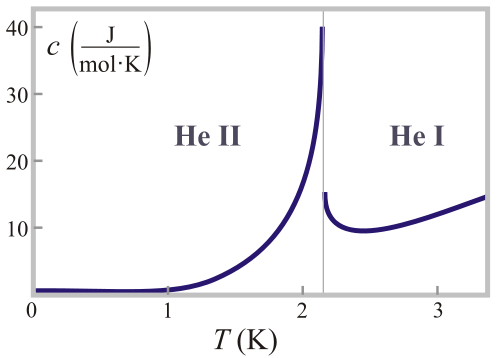
\includegraphics[width=0.3\textwidth]{lambda.png}
	\caption{Diagram showing the discontinuity in the heat capacity of liquid helium. Image courtesy of Wikimedia Commons.}
	\label{fig:lambda_point_helium}
\end{figure}

Like gravity, phase transition are phenomena which have long been observed, but only recently have they been understood scientifically. The freezing, melting, and evaporation of water has long been central to human life, controlling the availability of food and the need for shelter, but only in the past two centuries has any real effort been put into a scientific understanding of how matter transitions between these phases. The first serious attempt to understand this type of phenomenon was undertaken by Charles Caignard de la Tour in 1822. In his study, he classified the 'solid $\leftrightarrow$ liquid $\leftrightarrow$ gas' phase transitions of alcohol according to the Temperature, Pressure, and Volume at which they occurred \cite{phase_history}. Later, in 1873, Josiah Willard Gibbs built on this work to introduce the concept of the phase diagram\cite{phase_history, gibbs}. With this diagram came the notion that phase transitions could be understood from a purely thermodynamic transition. And, with the discovery of the ferromagnetic phase transition by Peter Curie in 1895 (along with its formal description by Peter Weiss in 1907), the race was on to find and classify phase transitions in a wide variety of systems. However, it wasn't until the discovery of the phase transition of liquid helium to a superfluid state that a solid classification system was able to take hold. It was observed experimentally that, during this transition, there was no latent heat and no visible boundary between the two phases \cite{phase_history}. Instead, it was found that there was a discontinuity in the second derivative of the free energy of the system, which showed itself in the famous lambda plot of heat capacity vs. temperature (Figure \ref{fig:lambda_point_helium}). This observation spurred Ehrenfest to introduce the first comprehensive classification system for phase transitions. The system was constructed around the 'order' of the discontinuity of the free energy of the system. Classically known phase transitions (water $\leftrightarrow$ ice, etc.) as well as others like the ferromagnetic transition of iron studied by Weiss and Curie are classified as first order phase transitions, while the newly discovered HeI $\leftrightarrow$ HeII transition is a second order transition. This classification scheme was soon validated, as superconductivity was proven to accompany the helium superfluid transition in the second order category. Landau built on this classification system to create much of the theory of phase transitions we still use today \cite{manual}.

We study an example of both a first and a second order transition in this lab. The first order transition we examine is the ferroelectric transition of BaTiO$_3$. This is quite similar to the ferromagnetic transition in 

\section{Review of Previous Work}

\section{Experimental Setup}

Our experimental setup consists of three main components: the lock-in amplifier, the sample chamber, and (during the resistance measurements) the limiting resistor.

\subsection{Resistance Measurements}

\subsubsection{Four Probe Method}

\subsection{Capacitance Measurements}

\subsection{Calibration and Measurement of Internal Resistance of Lock-In Amplifier}

\subsection{Preparation of Samples}

In the course of this lab, we will make use of two different sample materials: Vanadium Dioxide (VO$_2$) and Barium Titanate (BaTiO$_3$). The Vanadium samples consist of a thin layer of VO$_2$ ($\sim 100~nm$) deposited on a silicon substrate. These Vanadium samples are pre-mounted on their electrical contacts, but we have prepared a Barium sample for our own use. Our goal with the Barium sample is to construct a parallel plate capacitor using silver paint on either side of a flat sample. In order to maximize the capacitance, in accordance with the known relation $C = \epsilon A/d$ where $\epsilon = k \epsilon_0$, we want to maximize the surface area of our sample and minimize its thickness. To that end, we chose the largest piece of Barium Titanate available and carved it down. We began by scraping thick layers of material off with a x-acto knife, and when the sample became sufficiently thin we switched to sandpaper to smooth the surface.

\begin{figure}[H]
	\centering
	\begin{subfigure}{0.22\textwidth}
		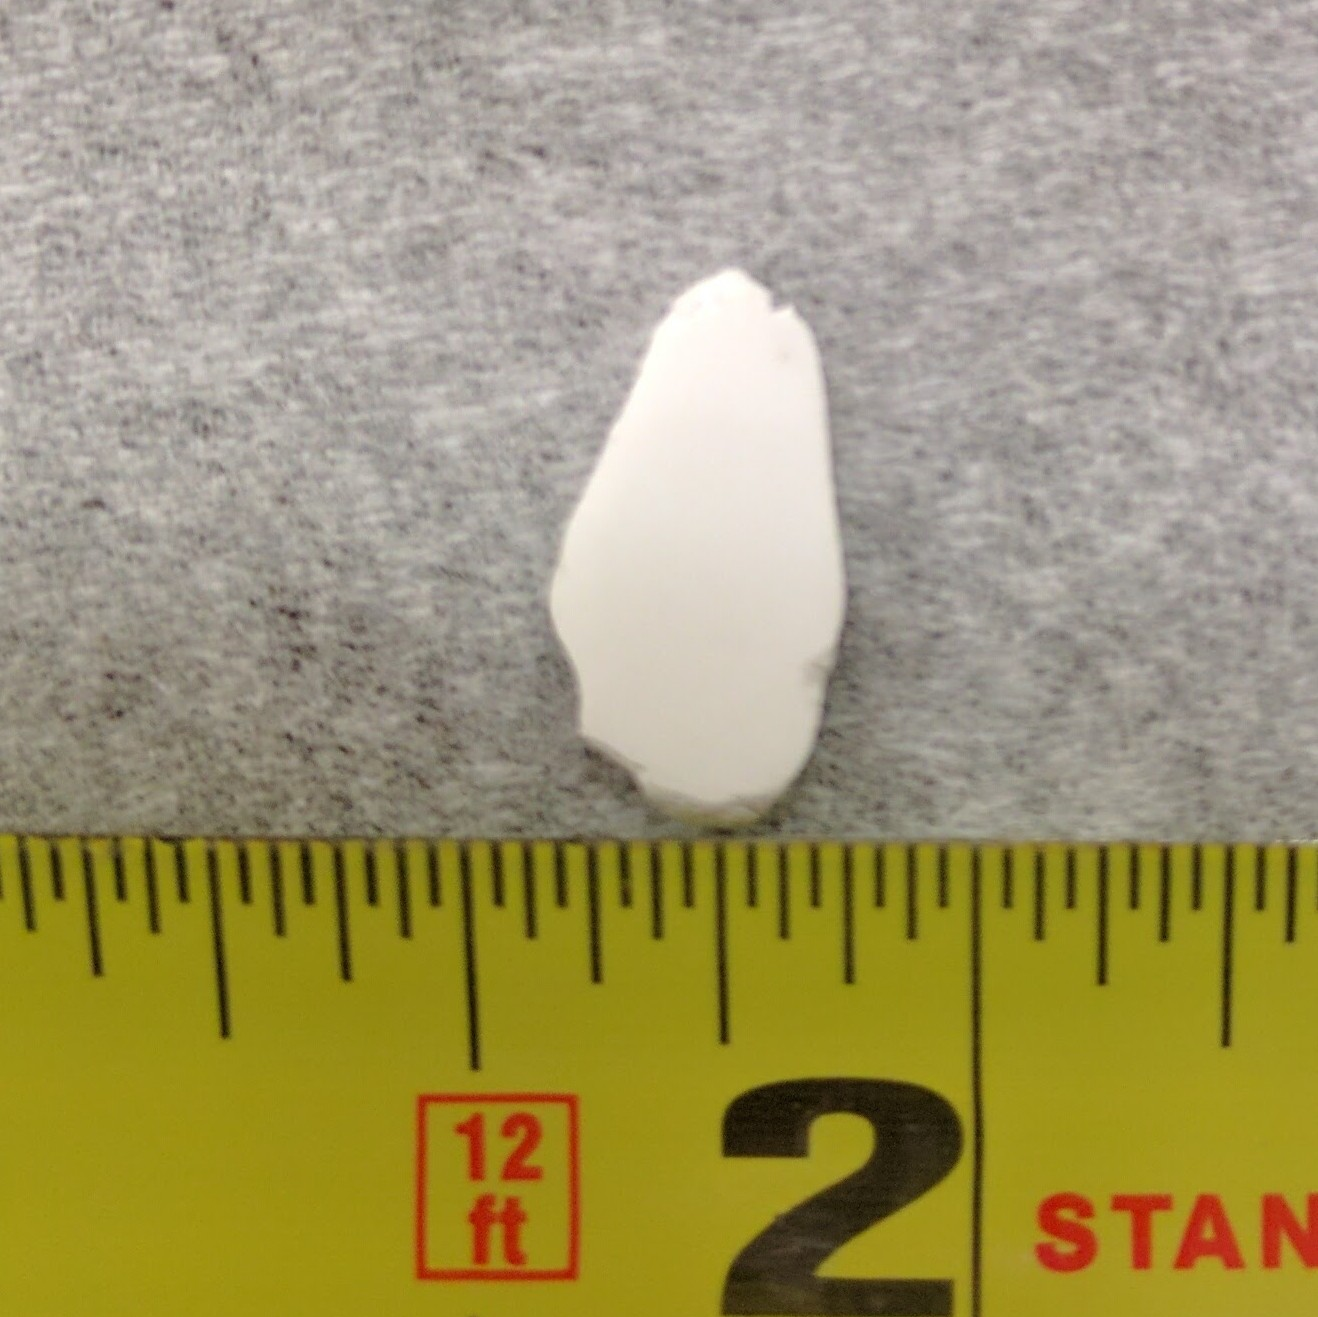
\includegraphics[width=1\textwidth]{sample_area.jpg}
		\caption{}
		\label{fig:sample:area}
	\end{subfigure}
	\begin{subfigure}{0.22\textwidth}
		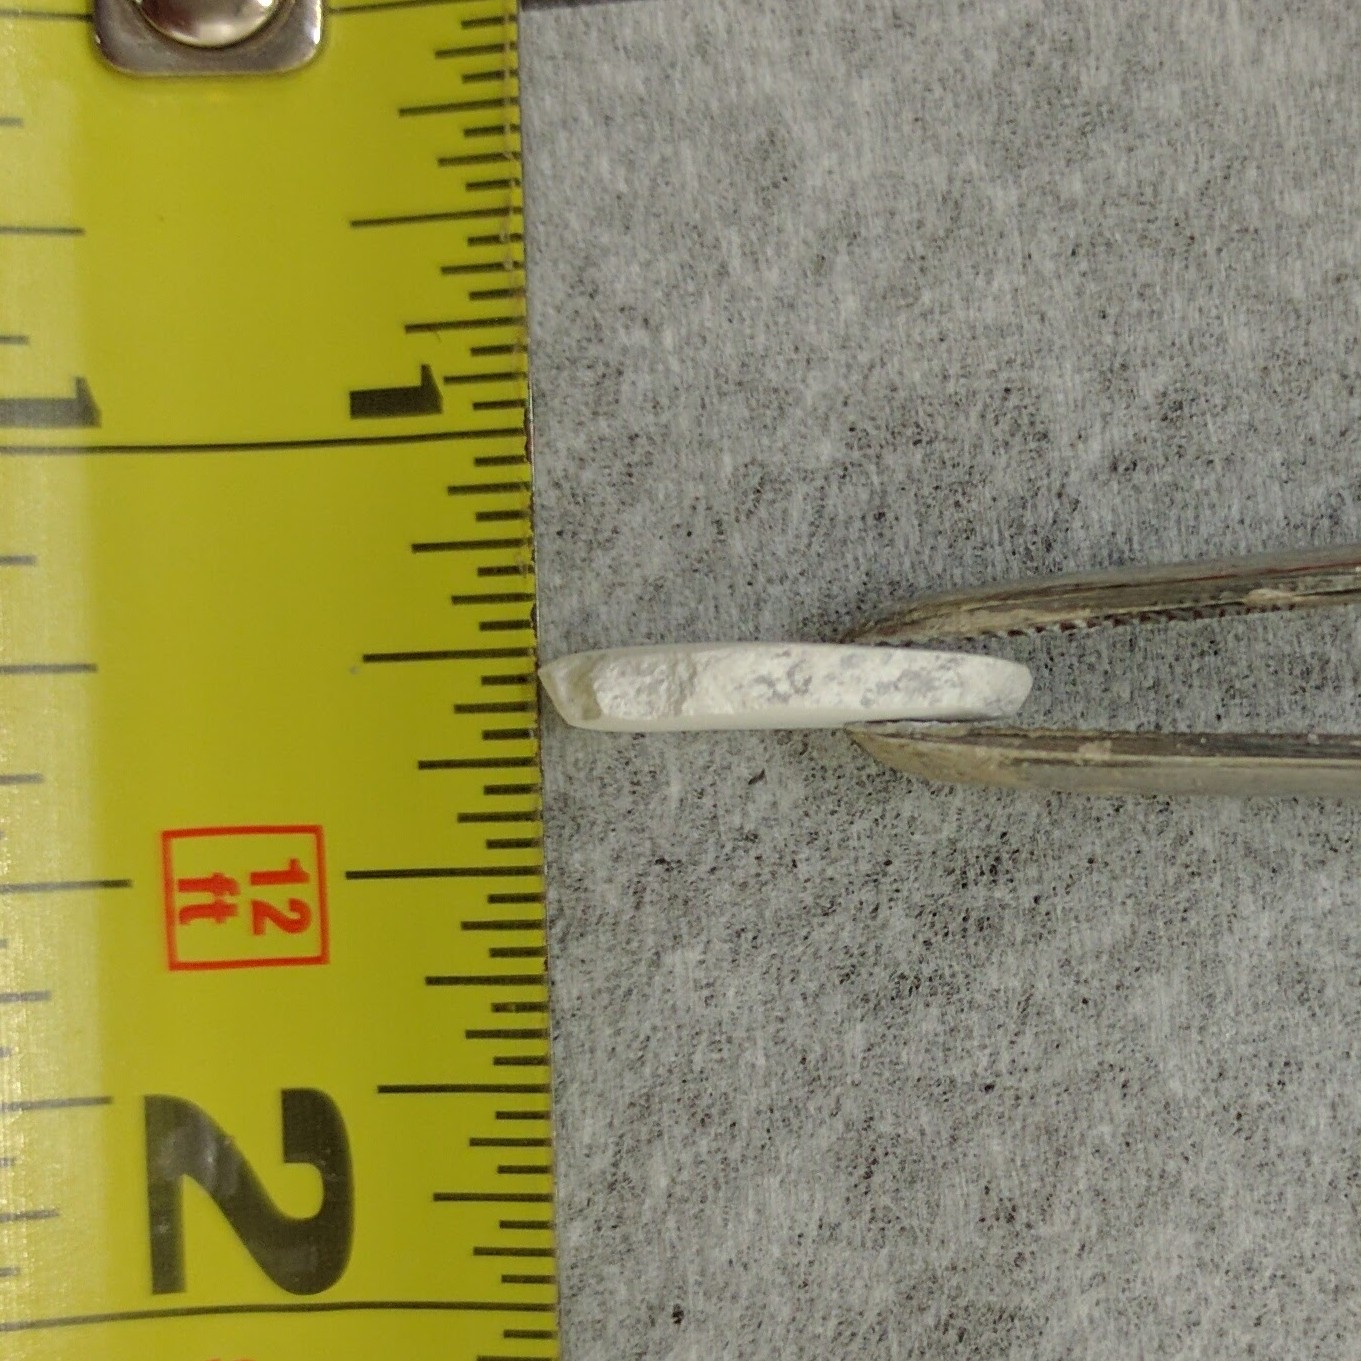
\includegraphics[width=\textwidth,angle=90]{sample_thickness.jpg} 
		\caption{}
		\label{fig:sample:thickness}
	\end{subfigure}
	\begin{subfigure}{0.22\textwidth}
		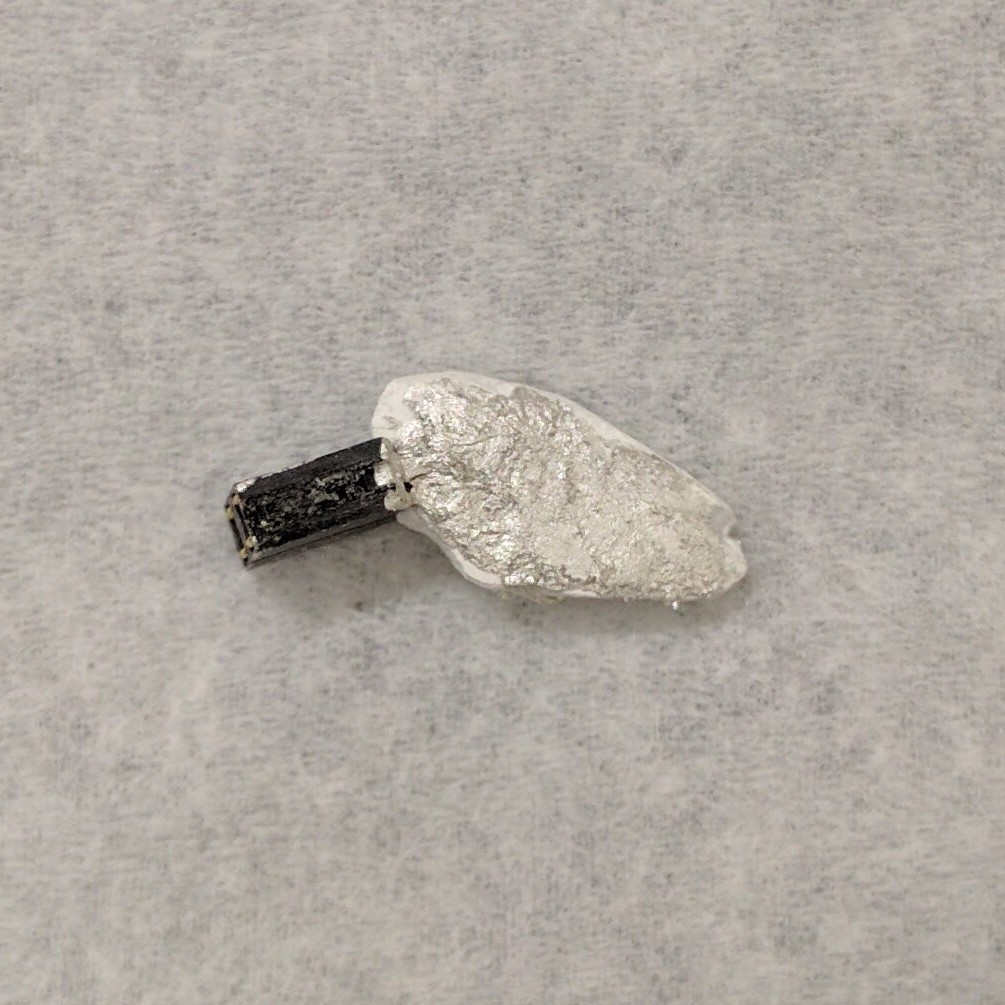
\includegraphics[width=\textwidth]{sample_complete.jpg}
		\caption{}
		\label{fig:sample:final}
	\end{subfigure}
	\begin{subfigure}{0.22\textwidth}
		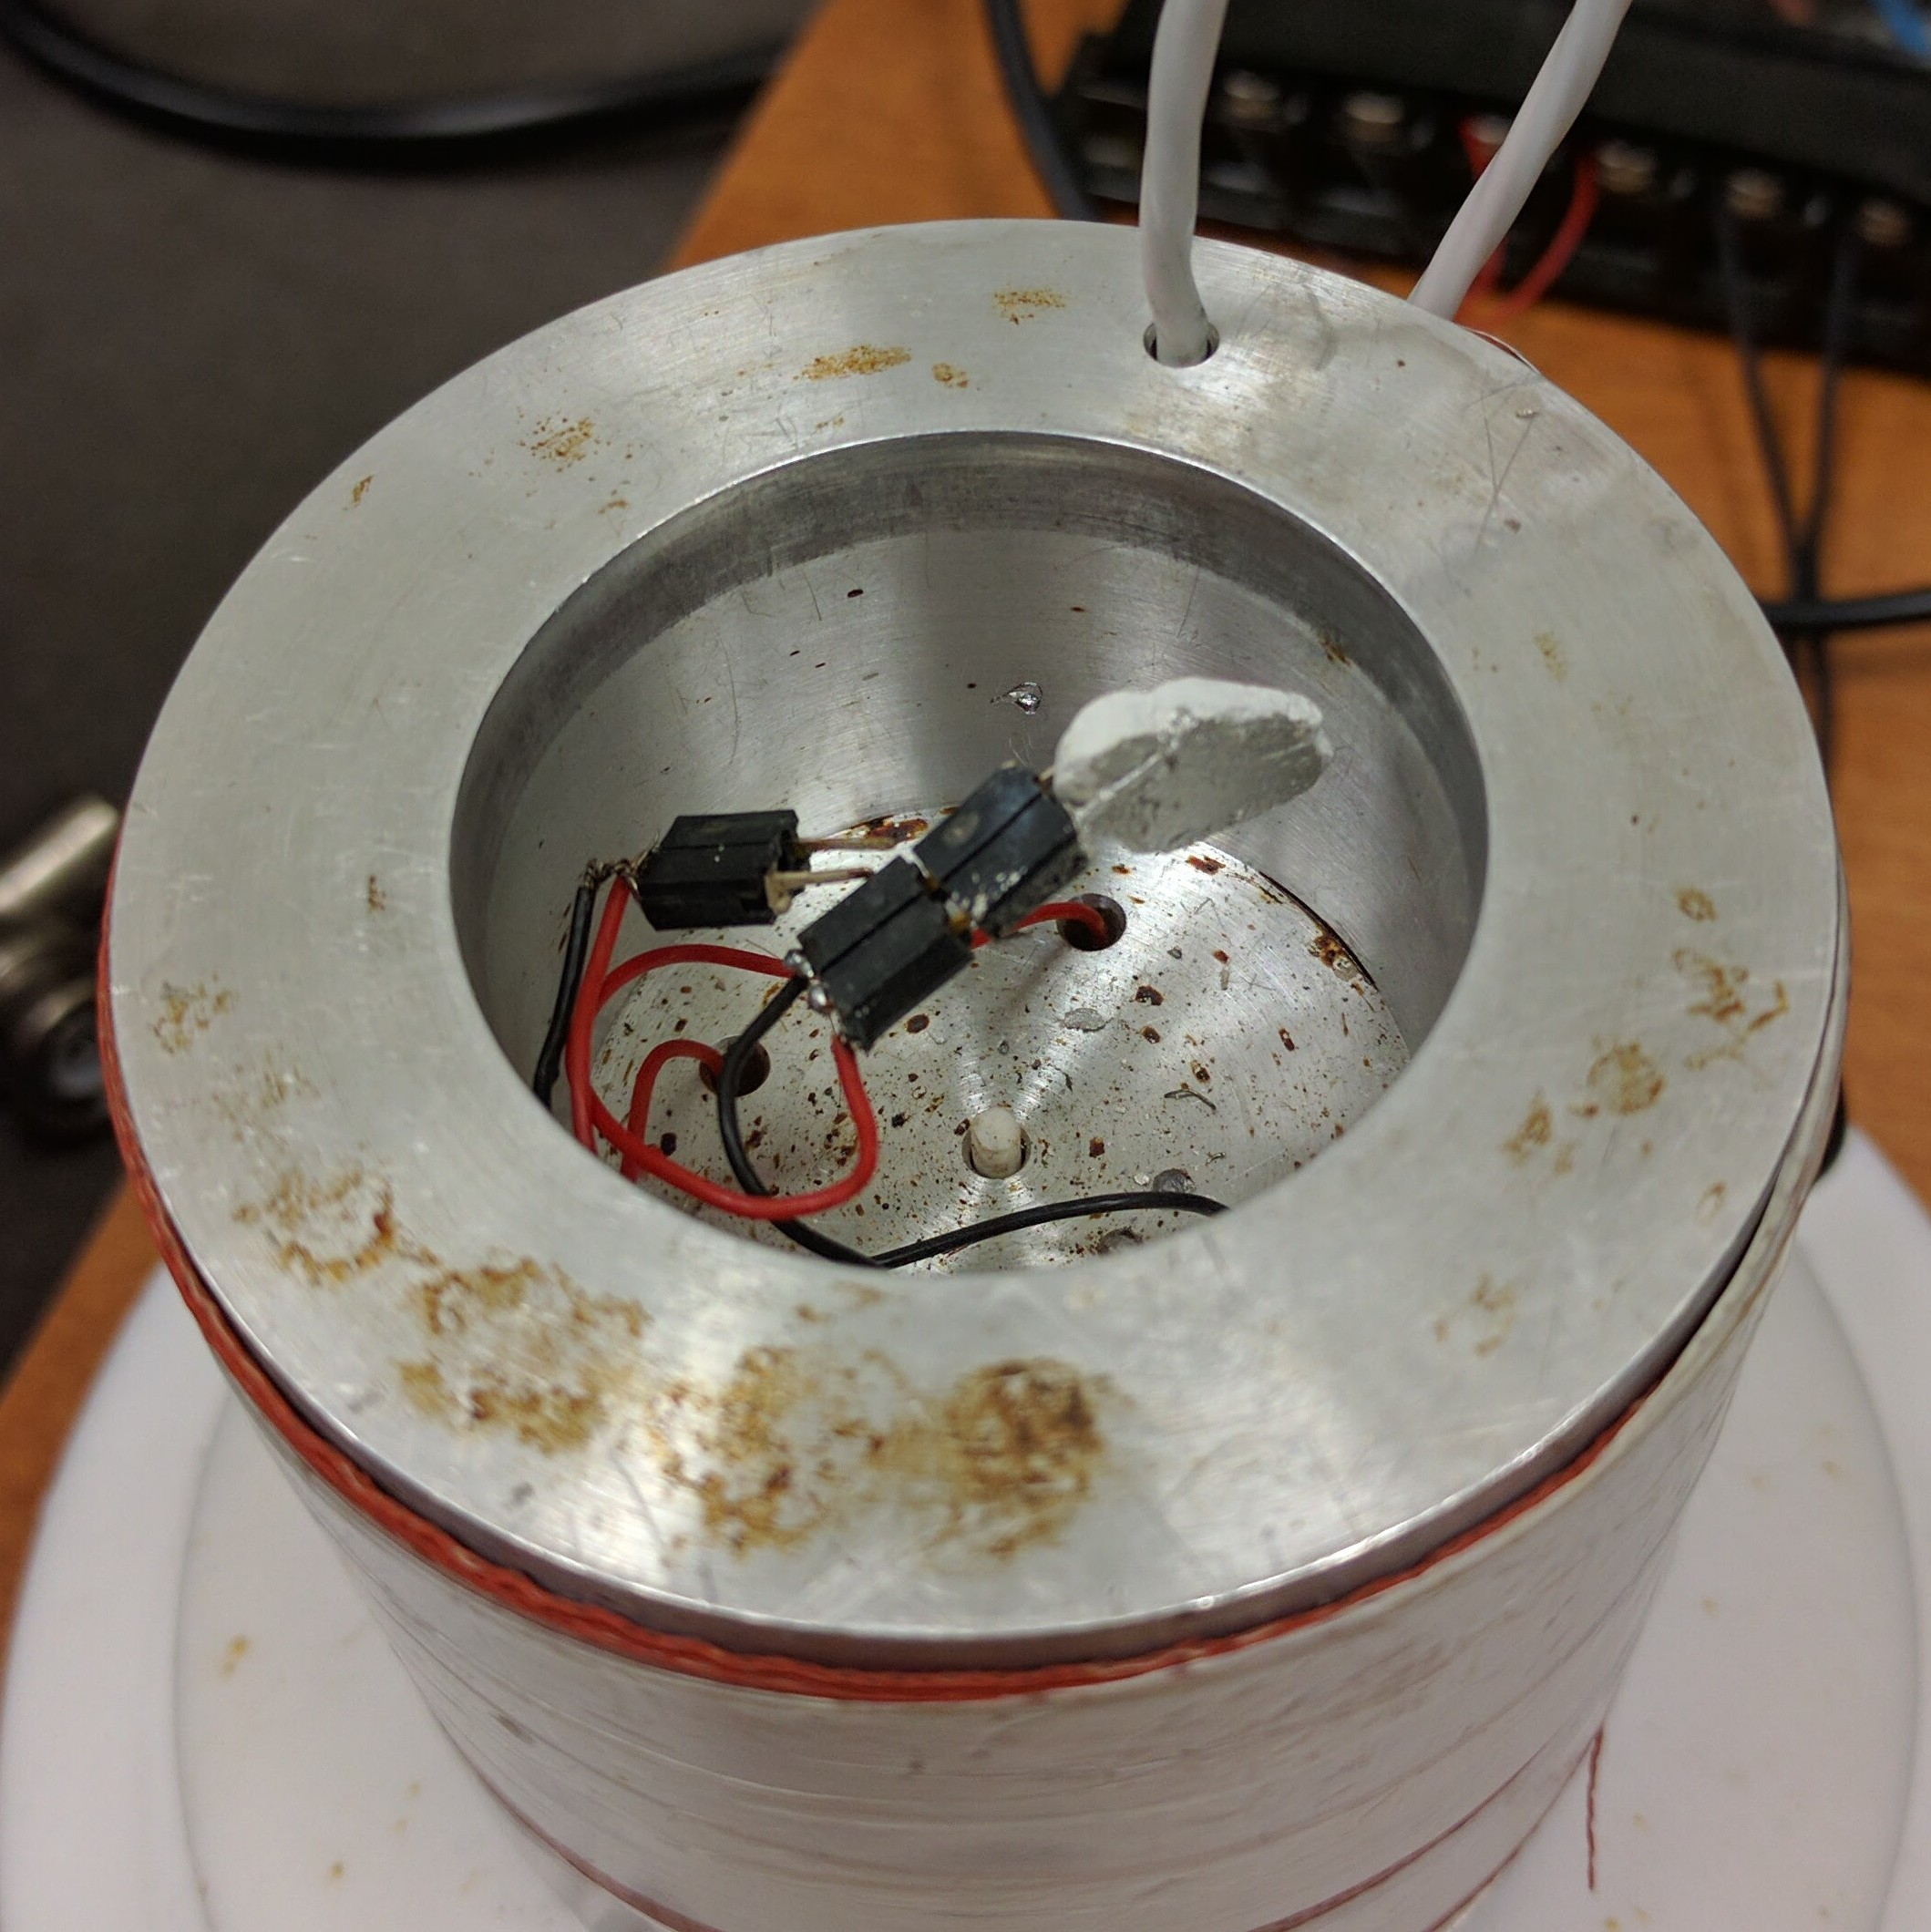
\includegraphics[width=\textwidth]{sample_inplace.jpg}
		\caption{}
		\label{fig:sample:inplace}
	\end{subfigure}
	\caption{Preparation of the Barium Titanate sample. Subfigures \ref{fig:sample:area} and \ref{fig:sample:thickness} show the images used to measure the thickness and the area of the sample. Subfigures \ref{fig:sample:final} and \ref{fig:sample:inplace} show the final sample, with the electrical connections attached by silver paint.}
	\label{fig:sample}
\end{figure}

Because we chose to maximize the area rather than creating a uniform geometric shape, whose area would have been simple to measure, we performed an indirect measurement of the area. Using a cell phone camera, we took an image with the sample and a ruler at the same distance. We used the photo editing tool GIMP to determine the surface area and thickness of the sample in pixels ($px$). We also measured the length of a section of the ruler to determine the $px$ to $mm$ conversion factor. From these measurements, we found that the area and thickness of the sample were:
\begin{gather}
	A_{sample} = 77.464 \pm 1.5470*10^{-2} ~mm^2  \nonumber \\
	d_{sample} = 1.8592 \pm 1.7820*10^{-3} ~mm	 \nonumber
\end{gather}
These values are consistent with our rough approximations taken during the lab period. From these we find that our equation for the capacitance of this sample is:
\begin{gather}
	\begin{align}
		C = \frac{\epsilon A}{d} & = k \epsilon_0 \frac{77.464 \pm 1.5470*10^{-2} ~mm^2}{1.8592 \pm 1.7820*10^{-3} ~mm} \nonumber \\
		& = k*(3.2384*10^{-13} \pm 3.1902*10^{-16})~F \nonumber \\
		& = k*(0.32384 \pm 3.1902*10^{-4})~pF \nonumber
	\end{align}
\end{gather}
where k is the relative dielectric permeability of the sample. 

\section{Measurements}

\section{Theoretical Model}

\section{Comparison of Theory and Experiment}

\section{Discussion and Conclusions}

\section{Author Contributions}

Both authors believe that the work for this project was split equally, and each offered valuable insight to every section of this report. However, the sections when divided up by principle author are as follows:

\noindent \textbf{Joshua LaBounty}:
\begin{enumerate}
	\item 
\end{enumerate}

\noindent \textbf{Thomas Krahulik}:
\begin{enumerate}
	\item Section 
\end{enumerate}

\noindent Lab time was also split equally, with one partner often taking measurements while the other developed the analysis software used in this report.

\begin{thebibliography}{6}
	
	\bibitem{milissinos}
	A.C. Melissinos, Experiments in Modern Physics (Academic Press, NY, 1966).
	
	\bibitem{bevington}
	Philip R. Bevington and D. Keith Robinson, Data Reduction and Error Analysis 3rd edition (McGraw-Hill, 2003).
	
	\bibitem{manual}
	Mihaly, Laszlo and Gurvitch, Micheal. Phase Transitions: Metal-Insulator Transition in VO$_2$ and Ferroelectric Transition in BaTiO$_3$. (Stony Brook University, Nov. 14, 2014)
	
	\bibitem{phase_1}
	Hadley, P. Advanced Solid State Physics: Landau theory of second order phase transitions. (Institute of Solid State Physics, 2011). \url{http://lampx.tugraz.at/~hadley/ss2/landau/second_order.php}
	
	\bibitem{modern_apps}
	M. Gittrman, V. Halpern, “Phase Transitions; A brief account with modern applications” World
Scientific, (2004)

	\bibitem{physics_of_phase}
	P. Papon, J. Leblond, P.H.E. Meijer, “The Physics of Phase Transitions”, Springer, (2001)
	
	\bibitem{phase_2}
	V. Dobrosavljevic, “Introduction to Metal-Insulator Transitions” (2011), arXiv:1112.6166v1
	
	\bibitem{phase_history}
	Jaeger, G. The Ehrenfest Classification of Phase Transitions: Introduction and Evolution. Archive for History of Exact Sciences. (1 May 1998). doi:10.1007/s004070050021.
	
	\bibitem{gibbs}
	Gibbs, J.W. On the Equilibrium of Heterogeneous Substances. Connecticut Academy of Arts and Sciences, 1874. \url{https://archive.org/details/Onequilibriumhe00Gibb}

\end{thebibliography}

\begin{appendix}

\section{Validation of the $\chi^2$ Minimization in ROOT} \label{section:root}
For this experiment, we used ROOT, a c++ based data analysis software, to plot and fit functions to our data. To verify that ROOT calculates a correct value for $\chi^{2}$, we performed a hand calculation cross check with a simple set of data. The data set we used for this cross check was $\{ (11.0 \pm 0.0, 23.0 \pm 0.5), (14.0 \pm 0.0, 25.0 \pm 0.5), (20.0 \pm 0.0, 35.0 \pm 0.5), (25.0 \pm 0.0, 39.0 \pm 0.5) \}$. We plotted this data and fit it to a linear function $f(x) = [0] + [1]*x$. This plot is shown in Fig.~\ref{Fig:rootproof}.
\begin{figure}[H]
	\centering
	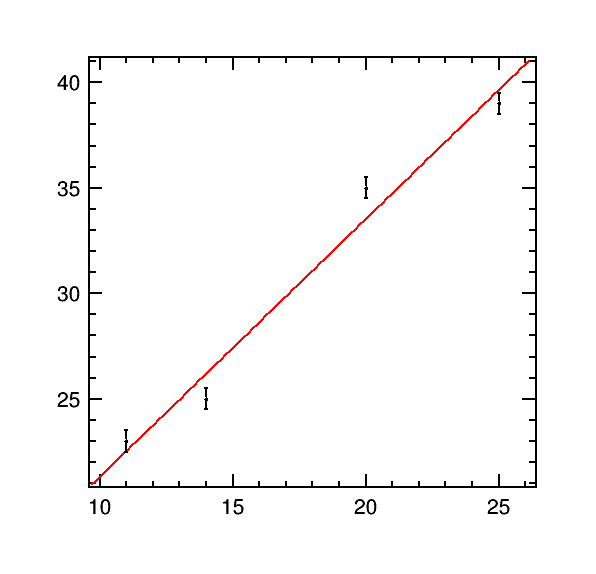
\includegraphics[width=0.4\textwidth]{rootproof.png}
	\caption{Sample Data Fitted to a Line}
	\label{Fig:rootproof}
\end{figure}
The function obtained from this fit was $f(x) = 9.11111 + 1.22222x$ with a chi-squared of $\chi ^{2} = 16.8889$. We then performed a hand calculation of the $\chi ^{2}$ using Eq.~\ref{eq:chisq}.
\begin{gather}\label{eq:chisq}
\chi ^{2} = \sum \frac{(f(x_i) - y_i)^{2}}{\sigma_i^2}
\end{gather}
When performing this hand calculation we also obtained a value of $\chi ^{2} = 16.8889$, verifying ROOT's ability to calculate $\chi ^{2}$.
\begin{align*}
\chi ^{2} =& \frac{(f(11.0) - 23.0)^{2}}{(0.5)^2} + \frac{(f(14.0) - 25.0)^{2}}{(0.5)^2} \\
&+ \frac{(f(20.0) - 35.0)^2}{(0.5)^2} + \frac{(f(25.0) - 39.0)^{2}}{(0.5)^2} \\
&= 16.8889
\end{align*}

\section{Analysis Code} \label{section:analysis_code}
All of the analysis code used for this lab can be found in the following git repository: 
\begin{verbatim}
https://github.com/jlabounty/SeniorLab/tree
/master/PhaseTransitions/
\end{verbatim}

\end{appendix}

\end{document}